\subsection{Declairing Things}

% Lazy induction definition
\begin{align*}
    \textbf{Base Case: } &\delta_1(i) = \Pi_i e_i(O_1)\\
    \textbf{Inductive Case: } &\delta_t(j) = \max_{1\leq i \leq N}[\delta_{t-1}(i)\psi(i,j)]\cdot e_j(O_t)
\end{align*}


% Lemmas, Theorems...
\begin{lemma}
    \label{prb:final}
    The algorithm is correct. 
\end{lemma}
\begin{proof}
I can ref myself \cref{prb:final}.
\end{proof}

  



\subsubsection*{Maths}
% Inline Maths
Maths in a $y=mx+c$.

% New line maths
word word word word 
\[y=mx+x\]
word word word

% Maths aligned
\begin{align*}
&O(k^3) + O(k^2) + O(nk^2) + O(k^3) + O(nk)\\
=& O(k^3) + O(nk^2)
\end{align*}

% Derivation with inline comments
\begin{align*}
    \sum_{x \in \Sigma^*} \beta_0(i) &= \sum_{i} \gamma_t{i} && \text{by definition}\\
    &= \gamma_t(i) && \text{cus it does}\\
    & = 1\\
\end{align*}

% Derivation with newline comments
\begin{align*}
    \shortintertext{By definition}
    \sum_{x \in \Sigma^*} \beta_0(i) &= \sum_{i} \gamma_t{i}\\
    \shortintertext{Because it does}
    &= \gamma_t(i)\\
    \shortintertext{Therefore}
    & = 1\\
\end{align*}


% Lots of maths, no align
\begin{gather*}
    \sum_{x \in \Sigma^*} \beta_0(i) = 1\\
    \sum_{i} \gamma_t{i} = 1\\
    \sum_{j} \xi_t(i,j) = \gamma_t(i)\\
    \sum_j \hat{m}_ij = 1\\
\end{gather*}


\[
    H = \begin{pmatrix}
    1 & 2 & 3\\
    a & b & c
    \end{pmatrix}
\]



\subsubsection*{Figures}
% Single figure
Ref the figure \ref{fig:em}.

\begin{figure}[h!]
    \begin{center}
        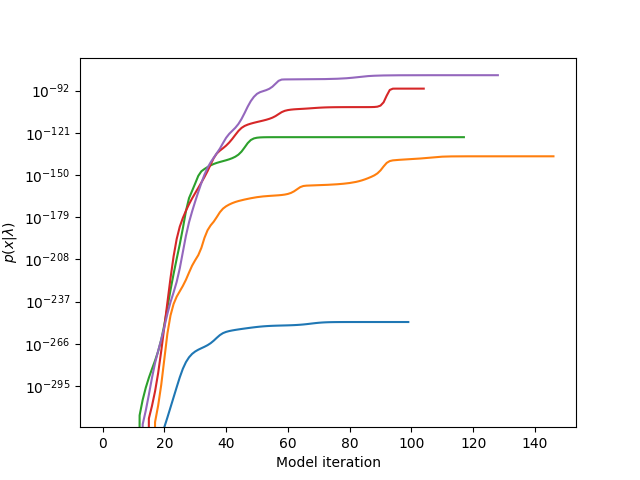
\includegraphics[width=.7\textwidth]{EM3.png}
        \caption{Words}
        \label{fig:em3}
    \end{center}
\end{figure}

% Double figure
\begin{figure}[h!]
    \begin{center}
        \begin{subfigure}{.5\textwidth}
            \begin{center}
                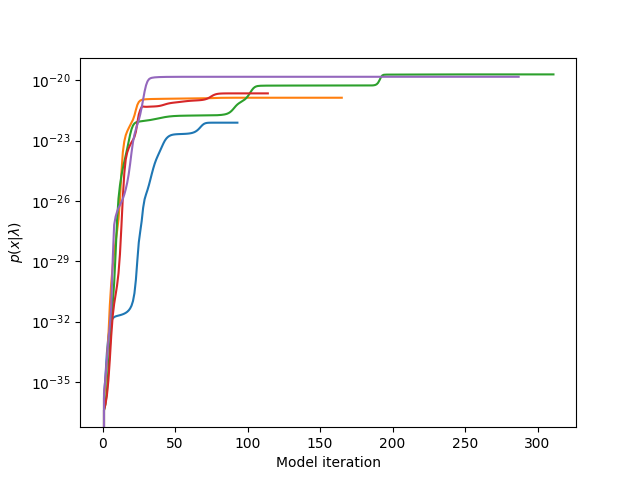
\includegraphics[width=.95\textwidth]{EM2.png}
                \caption{}
                \label{fig:em1}
            \end{center}
        \end{subfigure}%
        \begin{subfigure}{.5\textwidth}
            \begin{center}
                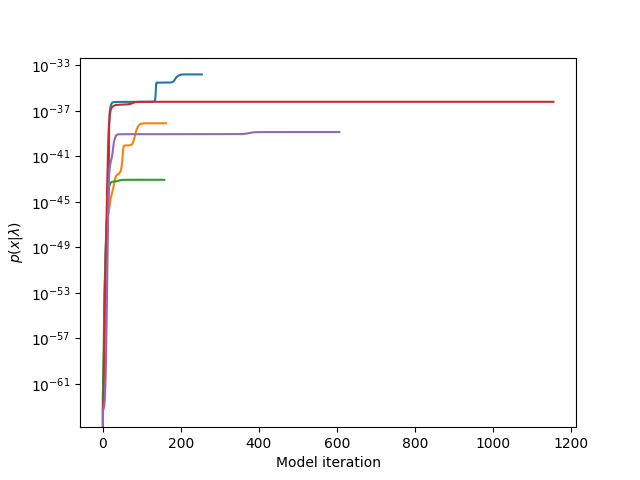
\includegraphics[width=.95\textwidth]{EM.png}
                \caption{}
                \label{fig:em2}
            \end{center}
        \end{subfigure}%
        \caption{words}
        \label{fig:em}
    \end{center}
\end{figure}

% Trees
\Tree [.
    [.
        [.
            [.
                c
                h
            ]
            a
        ]
        [.
            e
            f
        ] !{\qframesubtree}
        \qroof{\textit{${j, l, n}$}}.
    ] 
    \qroof{\textit{${b, d, g, i}$}}.
    \qroof{\textit{${k, m}$}}.
]

% Tree with branch labels
%\begin{tikzpicture}[
%    level distance=1.25cm,sibling distance=1cm,
%    edge from parent path={(\tikzparentnode) -- (\tikzchildnode)}]
% \Tree
% [.Mary
%     \edge node[auto=right] {B};
%     [.Alice 
%        \edge node[midway,left] {W};
%        [.$2,1$ ]
%        \edge node[midway,right] {J};
%        [.$0,0$ ]
%         ]
%     \edge node[auto=left] {C};
%     [.Alice
%         \edge node[midway,left] {W};
%      [.$0,0$ ]
%         \edge node[midway,right] {J};
%         [.$1,2$ ]
%         ]
% ]
% \end{tikzpicture}


% Table with headers
\begin{tabular}{cc|cc}
    &&\multicolumn{2}{c}{Alice}\\
    &&Wine&Juice\\
    \hline
    \multirow{2}{*}{Mary}&Beef&$(2,1)$&$(0,0)$\\
    &Chicken&$(0,0)$&$(1,2)$\\    
\end{tabular}

% Crazier picture
\begin{tikzpicture}[
    roundnode/.style={circle, draw=green!60, fill=green!5, very thick, minimum size=7mm},
    squarednode/.style={rectangle, draw=red!60, fill=red!5, very thick, minimum size=5mm},
    ]
    %Nodes
    \node                   (tl)                     {2};
    \node                   (tr)       [right=of tl] {1};
    \node[squarednode]      (bl)       [below=of tl] {3};
    \node[roundnode]        (br)       [right=of bl, below=of tr] {4};
    
    %Lines
    \draw[->] (tl.east) -- (tr.west) node[above, midway] {q};
    \draw[->] (bl.east) -- (br.west);
    
    \draw[->] (bl.east) -- (tr.west);
    \draw[->] (tl.east) -- (br.west);
    
\end{tikzpicture}


\begin{center}
    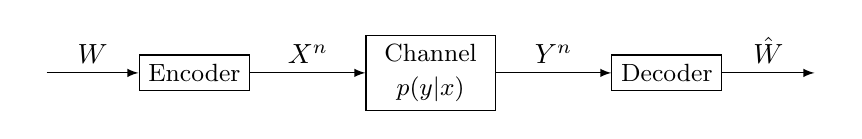
\begin{tikzpicture}[auto]
        \node (s) at (0,0) {}; %{\small{Message}};
        \node[draw] (e) at (2,0) {\small{Encoder}};
        \node[draw, text width=4em, text badly centered] (c) at (5,0) {\small{Channel} \small{$p(y|x)$}};
        \node[draw] (d) at (8,0) {\small{Decoder}};
        \node (r) at (10,0) {}; %{\small{Estimate}};
        
        \draw[-latex] (s) to node {$W$} (e);
        \draw[-latex] (e) to node {$X^n$} (c);
        \draw[-latex] (c) to node {$Y^n$} (d);
        \draw[-latex] (d) to node {$\hat{W}$} (r);
    \end{tikzpicture}
\end{center}

\begin{center}
    \begin{tikzpicture}[auto, xscale = 2, yscale = 2]
        \node (s0) at (0,3) {$0$};
        \node (s1) at (0,0) {$1$};
        \node (d0) at (3,3) {$0$};
        \node (d1) at (3,0) {$1$};
        
        \node (x) at (-1,1.5) {$X$};
        \node (y) at (4,1.5) {$Y$};
        
        \draw[-latex] (s0) to node[pos=0.3] {$p$} (d1);
        \draw[-latex] (s0) to node {$1-p$} (d0);
        \draw[-latex] (s1) to node[pos=0.3] {$p$} (d0);
        \draw[-latex] (s1) to node {$1-p$} (d1);
    \end{tikzpicture}
\end{center}

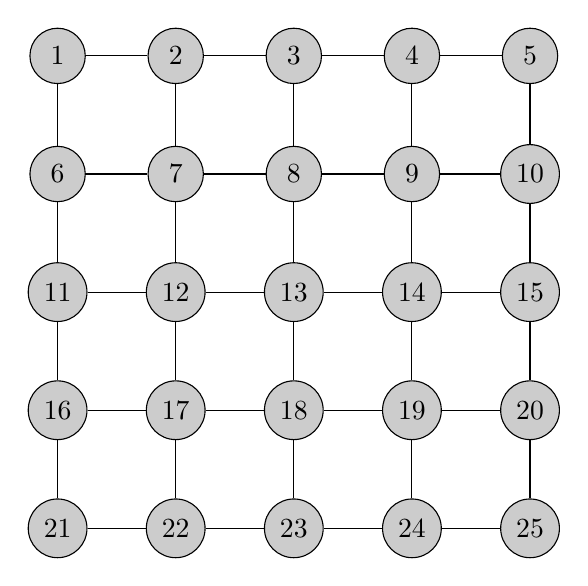
\begin{tikzpicture}[darkstyle/.style={circle,draw,fill=gray!40,minimum size=20}]
    \foreach \x in {0,...,4}
    \foreach \y in {0,...,4} 
        {\pgfmathtruncatemacro{\label}{\x - 5 *  \y +21}
        \node [darkstyle]  (\x\y) at (1.5*\x,1.5*\y) {\label};} 

    \foreach \x in {0,...,4}
    \foreach \y [count=\yi] in {0,...,3}  
        \draw (\x\y)--(\x\yi) (\y\x)--(\yi\x) ;

\end{tikzpicture}

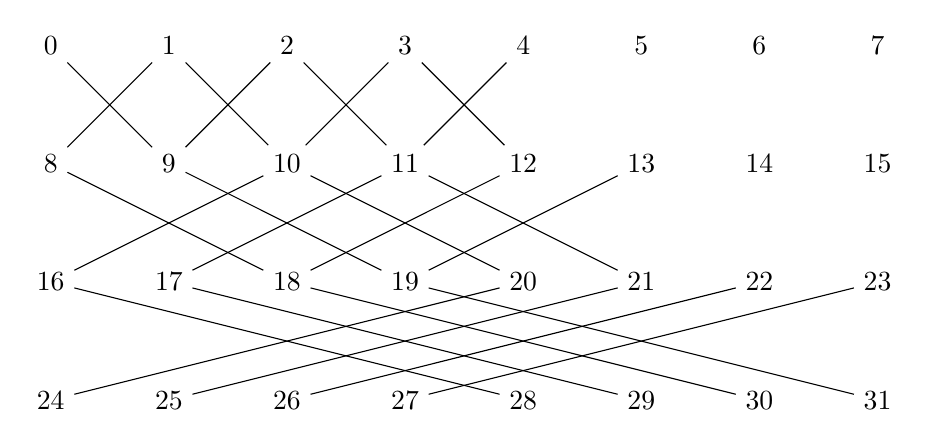
\begin{tikzpicture}[auto]
    \pgfmathtruncatemacro{\width}{8}
    \pgfmathtruncatemacro{\height}{4}
    \pgfmathtruncatemacro{\widthL}{\width-1}
    \pgfmathtruncatemacro{\heightL}{\height-1}

    \foreach \x in {0,...,\widthL}
    \foreach \y in {0,...,\heightL} 
    {
            %\pgfmathtruncatemacro{\y}{(\i - 1) / 5}
            %\pgfmathtruncatemacro{\x}{\i - 5 * \y}
            \pgfmathtruncatemacro{\label}{\x + \width * (\heightL - \y)}
            \node (\label) at (1.5*\x,1.5*\y)
            {\label};
    }
    
    % Horizontal connections
    
    \pgfmathtruncatemacro{\heightLL}{\heightL-1}
    \pgfmathtruncatemacro{\widthH}{\width/2-1}
    \foreach \y in {0,...,\heightLL}
    %\pgfmathtruncatemacro{\x}{\i}
    \foreach \i in {0,...,\widthH}
    {
            \pgfmathtruncatemacro{\x}{\i}
            \pgfmathtruncatemacro{\ox}{mod(\x + 2^\y, \width)}
            \pgfmathtruncatemacro{\oy}{\y+1}
            \pgfmathtruncatemacro{\tl}{\x + \width* \y}
           \pgfmathtruncatemacro{\tr}{\ox + \width* \y}
           \pgfmathtruncatemacro{\bl}{\x + \width* \oy}
           \pgfmathtruncatemacro{\br}{\ox + \width* \oy}
           %\draw (\cur) -- (\next);
           \draw (\tl) -- (\br);
           \draw (\bl) -- (\tr);
    }
    
    % Vertical connections
    %\foreach \start in {1,...,20}
    %{
    %    \pgfmathtruncatemacro{\down}{\start+5}
    %%    \draw (\start) -- (\down);  
    %}
    
\end{tikzpicture}



\subsection{Layout}
\newcommand{\splitPage}[2]{
\begin{minipage}{0.2\textwidth}
    #1
    \end{minipage} \hfill
\begin{minipage}{0.9\textwidth}
    #2
    \end{minipage}
}

\splitPage{
    something on the left
}{
    something on the right
}



\subsection{Pseudo code}
\begin{algorithm}[H]
    \SetAlgoLined
    \KwResult{ $\pi_C = S_1, S_2, \cdots, S_r$ }
     set $Q$ as empty queue\;
     set $\pi_C = \emptyset$\;
     \tcc{iterate over all training examples}
     \While{$Q$ is not empty}{
        dequeue command $p \equiv q$ from $Q$\;
        let $S_p, S_q$ be $S[setID[p]]$ and $S[setID[p]]$ respectively\;
        \If{$S_p\neq S_q$}{
          let $L$ be the shorter of $L_{setID[p]}$ and $L_{setID[q]}$\;
          \For{ each implication $u \equiv v \implies x \equiv y$ in L}{ 
           \If{one of $u$ and v is in $S_p$ and the other is in $S_q$}{
               add command $x \equiv y$ to $Q$\;
           }
          }
          append $L_{setID[q]}$ to $L_{setID[p]}$\;
         }
       }
    
     \caption{Partition Step}
    \end{algorithm}